\chapter{Materials and methods}
\section{DCE-MRI renography}
When the Contrast Agent is injected into the bloodstream, is starts its journey via the organism. It travels  through the abdominal aorta, which branches  into the left and right renal arteries supplying the kidneys with the blood.  

First, the CA reaches the renal cortex, where a portion of it is filtered by the glomerulus from the blood to the Bowman's capsule in the process of glomerular filtration. Next, it is passed by the renal tubule to the renal medulla to finally be collected by the collecting system.   
Chemicals such as Gadolinium-based markers used in DCE-MRI that are freely filtered but neither reabsorbed nor secreted by the kidneys can be used for estimating the Glomerular Filtration Rate in quantitative DCE-MRI analysis.
\begin{comment}
This chapter describes in details the implemented method of the quantitative analysis of the kidney's function. Firstly, the subsequent steps of image processing and analysis are presented and the, the performance of the chosen PK models is compared. The aim is to chose the model, which would be the best for GFR estimation and to draw a conclusion whether it can be considered a robust and reliable method for future applications. 
\end{comment}

This part of the thesis describes in details the implemented method of the quantitative analysis of the kidney's function from DCE-MRI. The chapter leads the reader through the subsequent steps of image processing and analysis to finally compare the performance of the chosen PK models. The aim is to choose the model, which allows for obtaining the best results for GFR estimation on the given data and to draw a conclusion if it can be considered a robust, reliable method for the future applications. 

\section{DCE-MRI acquisition}
The dataset used in this project consists of forty DCE-MRI sequences. Each of the twenty healthy, non-smoking participants underwent two MRI examinations at a~time interval of 7 days.
Gd-DOTA (\textit{gadoteric acid}), which is a gadolinium-based CA,  at a dose of 0.025\,mmol/kg was administrated as a bolus injection at 3\,ml/s in an antecubital vein followed by a 20\,mL saline flush.
The examinations were performed on the 32 channel 1.5\,T whole-body scanner (Siemens Magnetom Avanto \cite{simens}) with a gradient strength\,=\,45\,mT/m and slew rate\,=\,200\,mT/m/ms using a~standard six-channel body matrix coil and table-mounted six-channel spine matrix coil for signal reception.
The 74 volumes, each consisting of 30 slices, covering the kidneys and the aorta were continuously acquired every 2.3\,s for approximately 6\,min in coronal-oblique plane.
The acquisition matrix was 192\,$\times$\,192 whereas the voxel size was equal to 2.2\,$\times$\,2.2\,$\times$\,3\,mm$^3$.
The parameters of the used spoiled gradient recalled 3D FLASH pulse-sequence with echo time, $TE=0.8$\,ms, repetition time, $TR=2.36$\,ms, flip angle, $\alpha= 20^{\circ}$.

More information about the acquisition of DCE-MRI data used in this project can be found in \cite{eikefjord2017dynamic}.
A few frames of the sample raw DCE-MRI sequence are shown in Figure~\ref{fig:set}.
\newpage

\begin{figure}[H]
%\vspace{2.5cm}
\captionsetup[subfigure]{labelformat=empty,textformat=simple}
	\centering
	\subfloat[$t_0$]{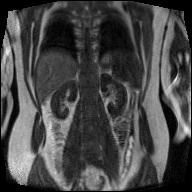
\includegraphics[height=0.26\linewidth]{img/preview/00}}\quad
		\subfloat[$t = 9\,Tp$]{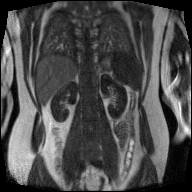
\includegraphics[height=0.26\linewidth]{img/preview/09}}\quad
			\subfloat[$t  = 12\,Tp$]{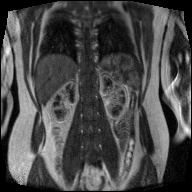
\includegraphics[height=0.26\linewidth]{img/preview/12}}\vspace{-4pt}
			
			
			\subfloat[$t  = 16\,Tp$]{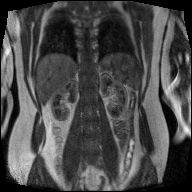
\includegraphics[height=0.26\linewidth]{img/preview/16}}	\quad		
			\subfloat[$t  = 18\,Tp$]{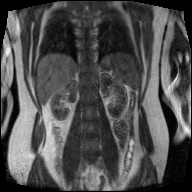
\includegraphics[height=0.26\linewidth]{img/preview/18}} \quad
		\subfloat[$t  = 22\,Tp$]	{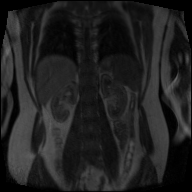
\includegraphics[height=0.26\linewidth]{img/preview/22}}\vspace{-4pt}
		
		
		\subfloat[$t  = 26\,Tp$]{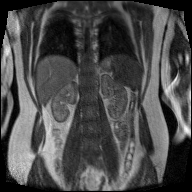
\includegraphics[height=0.26\linewidth]{img/preview/26}} \quad
			\subfloat[$t  = 30\,Tp$]{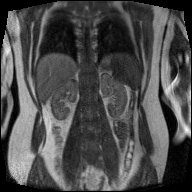
\includegraphics[height=0.26\linewidth]{img/preview/30}} \quad
			\subfloat[$t = 34\,Tp$]{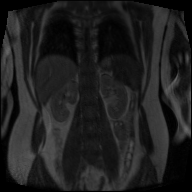
\includegraphics[height=0.26\linewidth]{img/preview/34}}\vspace{-4pt}
			
		\subfloat[$t  = 39\,Tp$]	{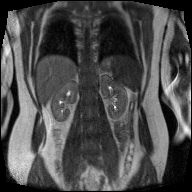
\includegraphics[height=0.26\linewidth]{img/preview/39}} \quad
	\subfloat[$t  = 55\,Tp$]{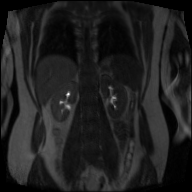
\includegraphics[height=0.26\linewidth]{img/preview/55}} \quad
	\subfloat[$t  = 73\, Tp$]{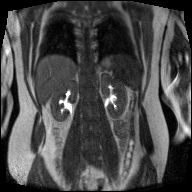
\includegraphics[height=0.26\linewidth]{img/preview/73}}
\vspace{0.2cm}
\caption[Sample DCE-MRI sequence of the healthy kidneys.]{Sample DCE-MRI sequence of the healthy kidneys. $Tp$ is a given time point. Firstly, the signal enhancement is observed in the renal cortex. Then, the tracer travels to the renal medulla and finally is collected by the collecting system}
\label{fig:set}
\end{figure}

\newpage
\section{GFR reference values}
Next to the DCE-MRI examinations, the participants had their GFR assessed by two chemical methods commonly used in the clinical practice: the \textit{serum-creatinine} (SCr) blood test and \textit{iohexol-GFR} tests. Creatinine is an endogenous indicator, which allows for estimating GFR from validated algorithms.
Iohexol in terms is an exogenous marker which is used for accurate GFR measurement. The clinical characteristics of all the participants are included in Table~\ref{tab:participants}

\begin{table}[h!]
\centering
\caption[Clinical characteristics of the participants]{Clinical characteristics of the participants \cite{eikefjord2017dynamic}}
\label{tab:participants}
\begin{threeparttable}
\rowcolors{2}{}{middleblue!30}
\renewcommand{\arraystretch}{1.25}
\begin{tabular}{L{7cm} R{4cm}}
	\toprule

 	Participants & 20\\
  	Gender (female/male) &16/4\\
  	Age (years) & 25 (20--38)\\
  	Height [m] & 1.71\,$\pm$\,0.07\\
  	Weight [kg] & 66.2\,$\pm$\,8.7\\
  	Body Mass Index (BMI) [kg/m\textsuperscript{2}] & 22.6\,$\pm$\,2.1\\
  	Body Surface Area (BSA) [m\textsuperscript{2}]& 1.77\,$\pm$\,0.14 (1.5--2.0) \\
  	Iohexol GFR [ml/min/m\textsuperscript{2}] &103\,$\pm$\,10 (87--125)\\
  	SCr GFR [ml/min/m\textsuperscript{2}] & 110\,$\pm$\,15 (81--128)\\
  \bottomrule

\end{tabular}
\begin{tablenotes}%
\footnotesize{}%
\item Values in parentheses are ranges.
\item Plus minus values are means $\pm$ Standard Deviations (SD).
    \end{tablenotes}
	\end{threeparttable}
\end{table}
\vspace{-0.1cm}
\section{Image processing and analysis}

\subsection{Motion correction}
One of the first fundamental problem encountered during DCE-MRI analysis is misalignment of the 3D volumes across time slices. This misalignment of organs is a result of the patient's respiratory motion as well as the heartbeat and bowel peristalsis and is unavoidable during examination. Studies have shown that even slight misalignment can lead to significant differences in intensity time-courses \cite{KidneySubsegmentation} and thus, motion correction of time series is essential for further analysis.

In order to remove 	the motion artifact, all files were motion-corrected across time points. For this purpose the R programming language for statistical computing and graphics was used \cite{R} together with the package ANTsR \cite{ANTsR}, which provides quantification tools for biomedical images. 

As an initial step, for every time series, the algorithm extracts the 3D volumes. Each extracted volume corresponds to the data obtained in one time point. Next, the average image of the temporal volumes is calculated, which serves as a target image for image registration. Every temporal volume is then aligned to it and at the end they are combined back together into the 4D time series.
As the misalignment concerns the inner structures, not the whole body and various organs have spatially variant geometric differences, the modality of choice was the  \textit{symmetric normalisation} algorithm (SyN), which is the non-rigid deformable transformation utilizing \textit{cross-correlation} (CC) as a similarity metric \cite{avants2011reproducible, avants2008symmetric, el2016current}. 

\subsection{Manual labelling}
In the next step, the labels of the whole left and right kidney were created. For this purpose the 3D volumes were extracted for each time frame and the slice with maximal signal enhancement of the kidneys was chosen (usually between 12--17 time slice). In this image, left and right kidney were manually delineated in coronal plane using the ITK-Snap software \cite{itk-snap}. Additionally, a few voxels of aorta (15--20) were labelled on maximal aortic enhancement time slice (9--10). So obtained labels were then combined and propagated across the time points. The sample labels are shown in Figure~\ref{fig:labels}.
All further analysis was implemented in the Python programming language~v.~3.6 \cite{python}.

\begin{figure}
\captionsetup[subfloat]{captionskip=0.5cm}
	\centering
	\subfloat[Labels of the left and right kidneys]{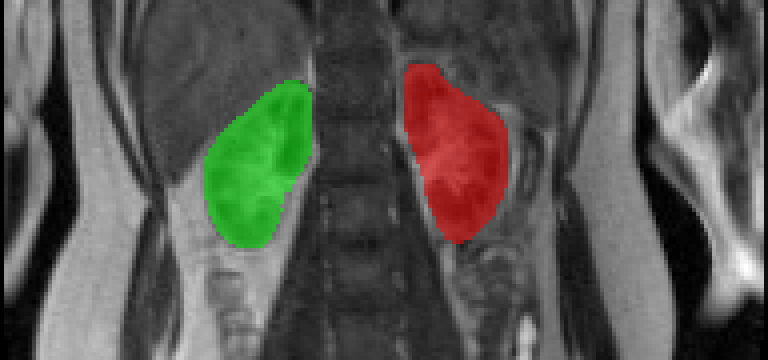
\includegraphics[width=0.48\textwidth ]{kidneys}}\hspace{0.02\textwidth}
	\subfloat[Label of the aorta]{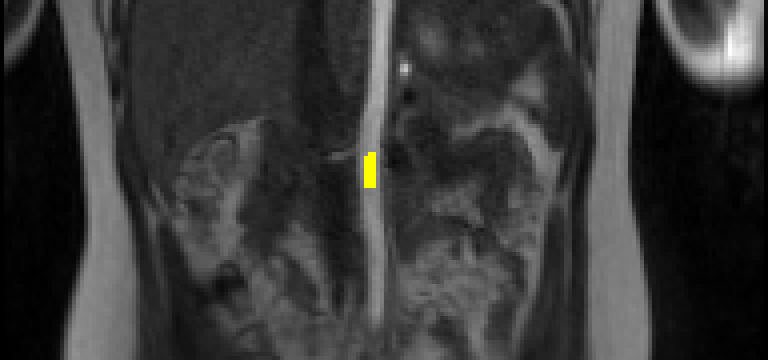
\includegraphics[width=0.48\textwidth]{aorta}}\\	
\vspace{0.5cm}
\caption[Sample labels of kidneys and aorta]{Sample labels of kidneys and aorta. Green and red are labels of the right and left kidney respectively, whereas yellow is the aorta label}
\label{fig:labels}
\end{figure}

\subsection{Pelvis region removal}
Due to the fact that glomerular filtration takes place in renal parenchyma, the region of pelvis had to be removed from further analysis. 

Resulting from the physiology of the process, the three renal compartments (cortex, medulla, pelvis) can be distinguished from each other on the basis of their time courses, as shown in Figure~\ref{fig:timecourses}. Depending on the compartment, the rapid enhancement of the signal occurs in different periods, which makes the shapes of the time intensity curves very unique.
From the Figure~\ref{fig:timecourses} it can be seen that the highest variation is observed between pelvis and two other renal compartments.
Consequently, it can be separated by unsupervised clustering.


\begin{figure}
	\centering
	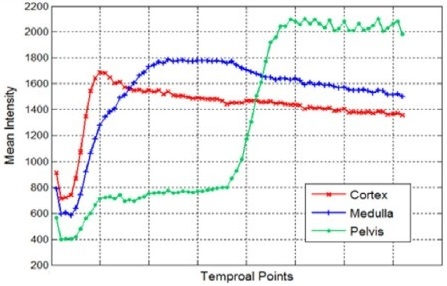
\includegraphics[width=10cm]{img/timecourses}
	\caption[Example kidney compartments timecourses]{Example kidney compartments timecourses \cite{KidneySubsegmentation}}
	\label{fig:timecourses}
\end{figure}


First of all, each voxel included in the label of the kidney was described by the vector of seventy-four features as follows:
\begin{equation}
\label{eq:voxel}
\mathbf{v_{ijk}} = [S(0),\; S(1),\;...\;,\; S(72),\; S(73)],
\end{equation}
where $S(n)$ is the value of signal intensity at the time point $n$.
\newpage

However, feature space of seventy-four dimensions is way too large for further analysis. High dimensionality of raw DCE-MRI data results in computational complexity, and thus memory and time consumption as well as numerical problems. What is more, it contains a lot of noise \cite{KidneySubsegmentation}. To overcome this problems, the \textit{principal component analysis} (PCA) \cite{pca} was applied.

PCA is a statistical procedure, which transforms the number of interrelated features into smaller set of uncorrelated variables. These so-called \textit{principal components} (PCs) are the linear combinations of the original variables \cite{dunteman1989principal}. As a result, after rotating the feature space, the first PC contains most variance, the last one the least and so on. In this way the dominant patterns are extracted, while the noise is reduced~\cite{pca, jolliffe1986principal}. Further, every of the PC is characterised by a ratio of \textit{explained variance}, which indicates the portion of the dataset’s variance lying along the axis of each PC~\cite{handson}.

Applying the theory to practice, each voxel belonging to the kidney, initially described by forty-four features was described by a number of PCs:
\begin{equation}
\label{eq:voxelpca}
\mathbf{v_{ijk}} = [PC1,\; PC2,\;...\;,\; PCn]  
\end{equation}
The amount of PCs, $n$, was chosen as a minimum number of dimensions required to preserve 95\% of the data's total variance so that the sum of the explained variances of  $n$ PCs was equal to at least 0.95 (usually between 4--6 PCs). The visual representation of the feature space with first three dimensions (PCs) for sample kidney is shown in Figure~\ref{fig:pca_plot}. Note that for better understanding, the clusters were already marked with different colors. 

\begin{figure}[H]
		\centering
		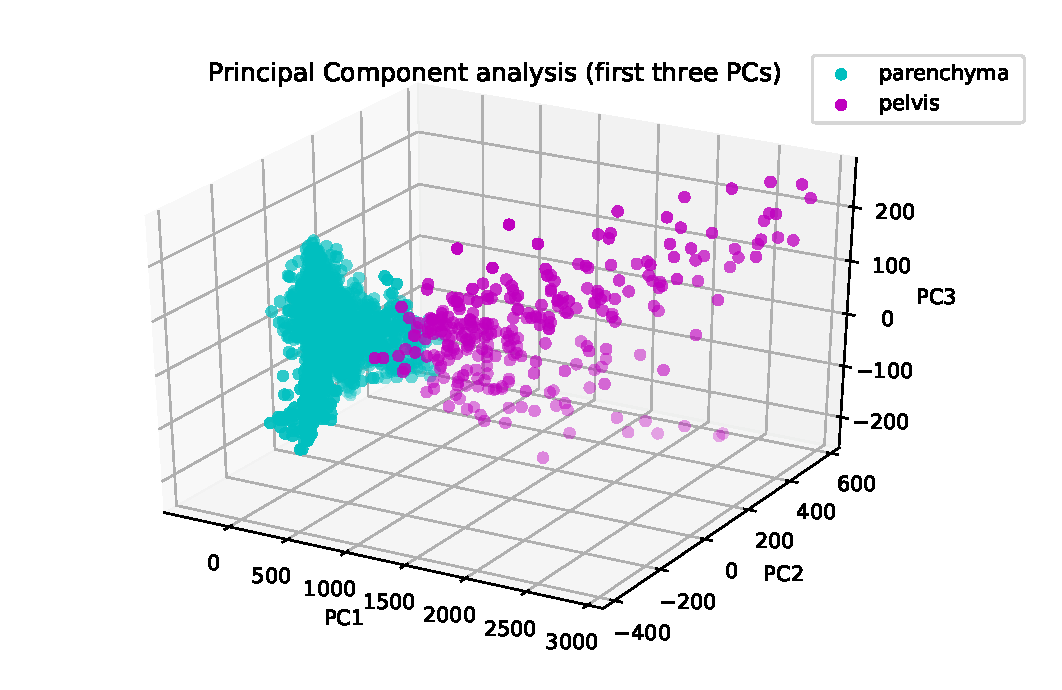
\includegraphics [height = 10cm]{pca}
		\caption [Principal Component Analysis for a sample kidney]{Principal Component Analysis for a sample kidney. The values in brackets are the ratios of explained variance for the given PCs. Note that the number of PCs was reduced to three for visualisation purpose}
		\label{fig:pca_plot}
	\end{figure}

To the dimensionally reduced data, the \textit{k-means clustering}} was applied in order to separate voxels into two groups: pelvis and renal parenchyma. 
The k-means is an unsupervised clustering algorithm aiming to divide the data into groups so that the diversity between the groups is maximised whereas the similarity within the single group is maximised  \cite{kmeans}. 

Given a data set $X=\{ \vec{x_1}...\vec{x_n}$\} in $m$-dimensional space (what actually corresponds to the $m$ features of a sample) the algorithm's objective is to minimize the square error function given by  \cite{kmeans, alsabti1997efficient}:

\begin{equation}
	\label{eq:kmeans}
	J = \sum_{j=1}^{k}\sum_{x_i \in S_j}(||x_i-c_j||)^2,
\end{equation}
where $||x_i-c_j||$ is  the Euclidean distance between a data point $x_i$ and the cluster centre $c_j$ of cluster $S_j$ from $k$ predefined clusters. It is achieved by the steps summarised in Algorithm~\ref{alg:kmeans}.

\vspace{16pt}
\begin{algorithm}[H]
\footnotesize
    \SetKwInOut{Input}{Input}
    \SetKwInOut{Output}{Output}
    \SetKwFunction{RandomlyChooseCentroids}{RandomlyChooseCentroids}
    \SetKwFunction{CalculateMeanOfPointsInCluster}{CalculateMeanOfPointsInCluster}
    \SetKwData{Centroids}{$(\vec{c_1}...\vec{c_k})$}
    \SetKwFunction{argminDistance}{argminDistance}
    
	\Input{number of clusters $k$,\\ set of points in $m$-dimensional space: $X=\{ \vec{x_1}...\vec{x_n}$\}}
	
    \Output{set of cluster labels of $X$: $L = \{l(\vec{x_i})\;i \in\{1...n\}\}$ ,\\ coordinates of cluster centroids: \Centroids}
    
    \BlankLine
    \BlankLine
    
    
	\DontPrintSemicolon
	\Centroids $\leftarrow$ \RandomlyChooseCentroids{$k$, $X$} \Centroids$\in X$\;
    
	\Repeat{none of \Centroids changes}{
\tcc {assign each data point to the closest centroid on the basis of Euclidean distance}
$l(\vec{x_i})\leftarrow$\argminDistance($\vec{x_i}$, $\vec{c_j}$) $j \in\{1...k\}$ \\
\Centroids$\leftarrow$  \CalculateMeanOfPointsInCluster{}  \tcc*{recalculate centroids} 
}
	\Return{$L$ , \Centroids} \tcc*{points divided into clusters} 
    
    
    \SetAlgoCaptionSeparator{.}
    \caption{K-means clustering}
    \label{alg:kmeans}
\end{algorithm}

\vspace{16pt}
To segment the kidney, the k-means algorithm was initiated with two clusters, $k$~=~2 and performed for points (kidney voxels) in $m$-dimensional space ($m$ is the number of PCs).
Further, for each of the identified clusters, the average time point, $T_{max}$ in which signal intensity reaches its maximum was calculated. 
Following the assumption that $T_{max\_pelvis}>T_{max\_parenchyma}$, the cluster with greater $T_{max}$ was marked as the pelvis and removed from the \textit{Region of Interest} (ROI).
The average time-intensity curves for two detected clusters in k-means clustering algorithm for sample kidney are presented in Figure~\ref{fig:clusters}. One can easily note that the wash-in phase in pelvis takes place much later than in renal parenchyma. The results of the segmentation in turn are shown in Figure \ref{fig:segmentation}.  
\vspace{1cm}

\begin{figure}[H]
%\captionsetup[subfloat]{captionskip=0.5cm}
	\centering
	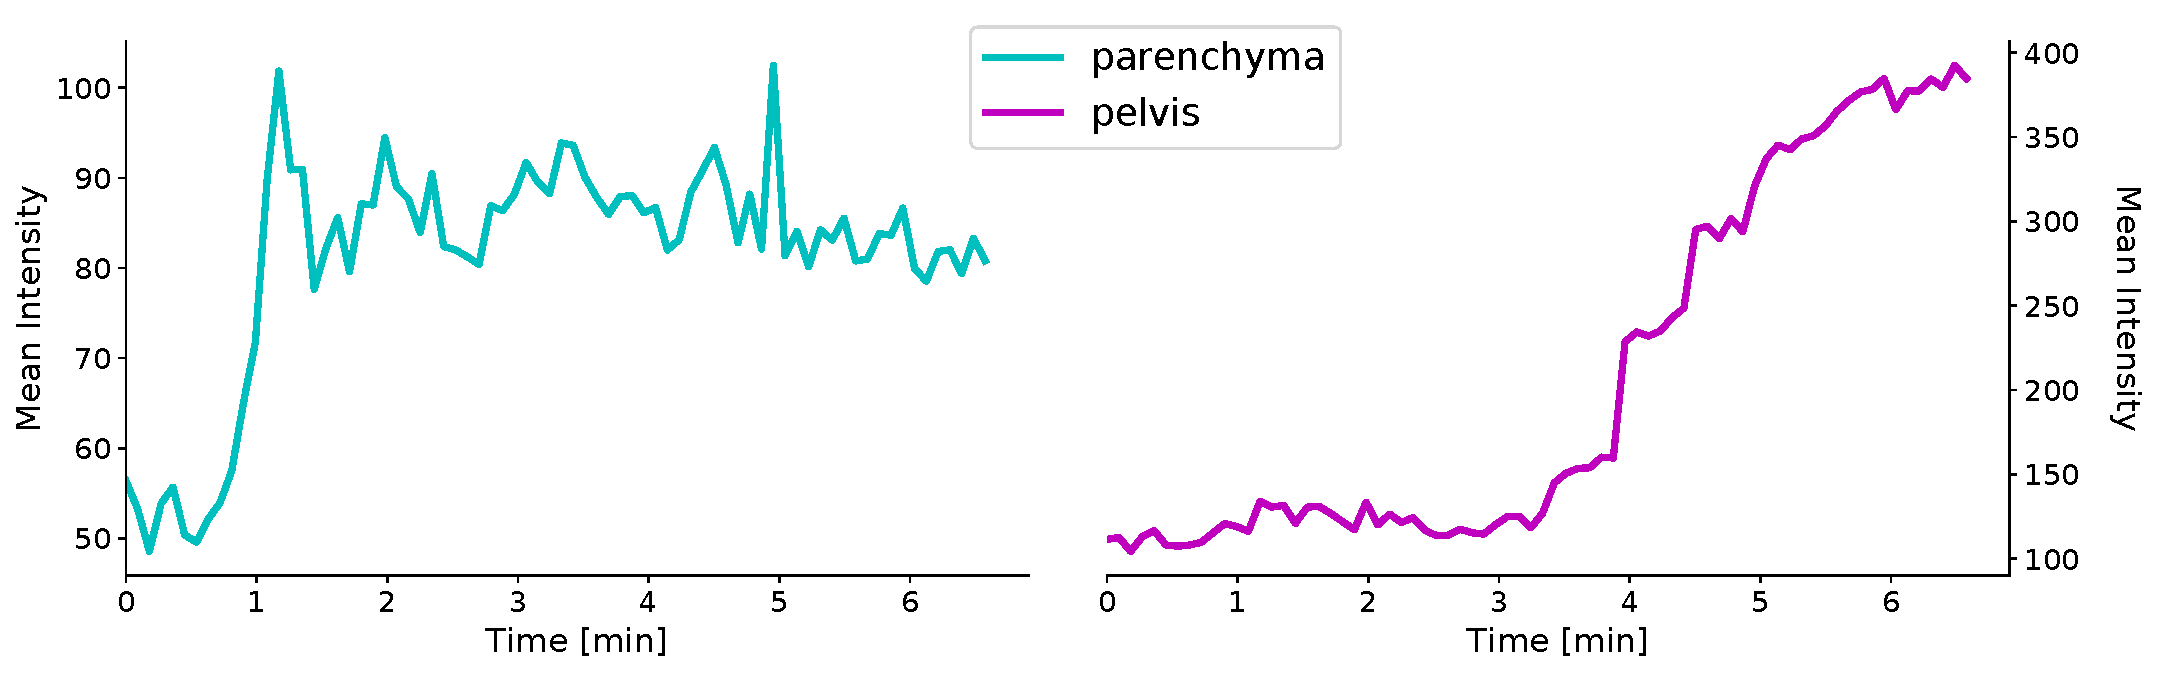
\includegraphics[width = \textwidth]{clusters}
	
\caption[Average time courses for two clusters detected in k-means algorithm]{Average time courses for two clusters detected in k-means algorithm performed for sample kidney}
\label{fig:clusters}
\end{figure}
\vspace{1cm}
\begin{figure}[H]
\captionsetup[subfloat]{captionskip=0.5cm}
	\centering
	\subfloat[Kidney segmentation]{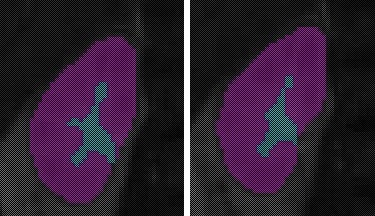
\includegraphics[width=0.48\textwidth ]{kidney_pelvis}}\hspace{0.02\textwidth}
	\subfloat[Renal parenchyma]{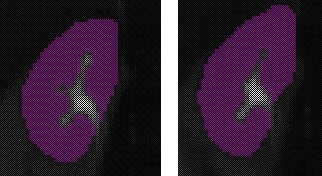
\includegraphics[width=0.48\textwidth]{no_pelvis}}\\	
\vspace{0.5cm}
\caption[Sample kidney segmentation with k-means clustering]{The results of the segmentation obtained with k-means clustering. Figure (a) shows two regions of a sample kidney: the pelvis (cyan) and the renal parenchyma (magenta); Figure (b) presents the kidney after pelvis removal. The images were intentionally presented at Time point $Tp$ = 73, when the enhancement of the pelvis is high, for better visualisation}
\label{fig:segmentation}
\end{figure}

\newpage
\subsection{Concentration-time curves}
Having labelled the proper ROI, the time has come for the principal part of the analysis, namely pharmacokinetic modelling.
The whole PK part was implemented in Python programming language from the scratch and no ready toolboxes for PK modelling were used.

All PK models used during quantitative DCE-MRI analysis call for determining both the tissue, $C_t(t)$, and blood plasma, $C_p(t)$, concentration as a~function of time. In our case, the $C_t(t)$ is the mean concentration in renal parenchyma, whereas the
$C_p(t)$, can be derived from the AIF, which is a concentration in a blood vessel feeding the kidney (aorta).
Thus, they were calculated in the next steps of the project.  

For each of the kidney, as well as for the aorta, the mean intensities of the voxels included in the particular labels were calculated at the each time point and the intensity time courses were plotted. Sample time courses are shown in Figure~\ref{fig:temporal_points}.

\vspace{50pt}
\begin{figure}[H]
%\captionsetup[subfloat]{captionskip=0.5cm}
	\centering
	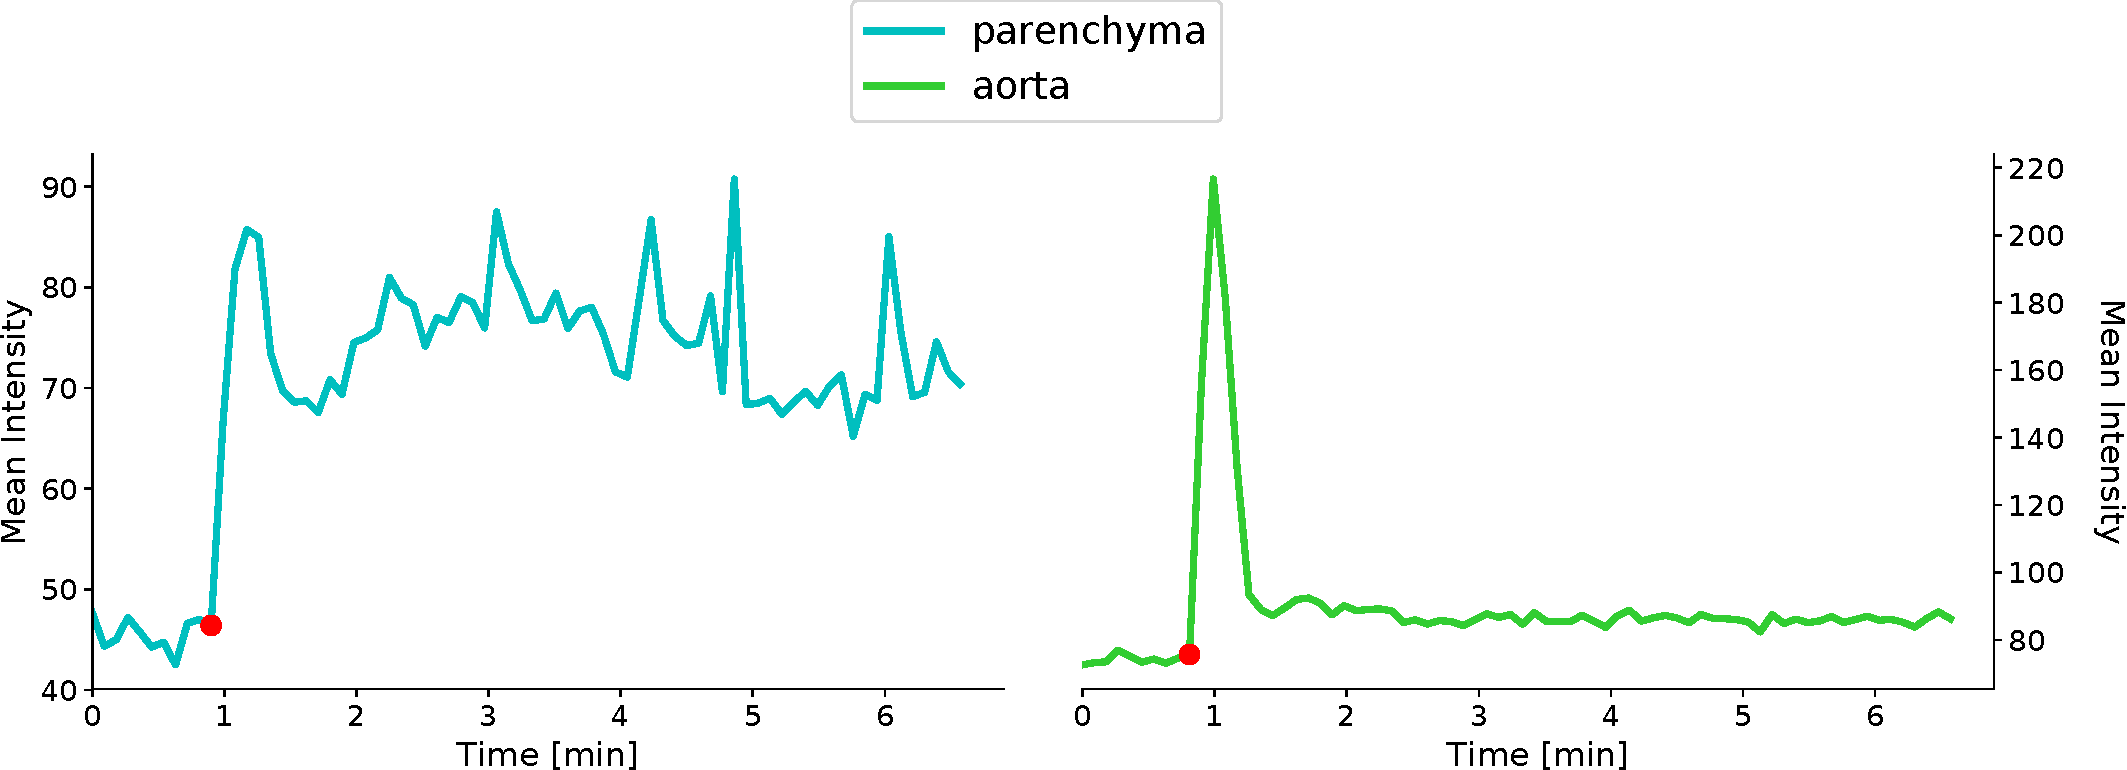
\includegraphics[width = \textwidth]{temporal_points}
	
\caption[Sample average time-intensity curves for a kidney and aorta with marked last points of the baseline]{Sample average time-intensity curves for a kidney and aorta. Red dot is $t_{baseline}$, the last point of the baseline}
\label{fig:temporal_points}
\end{figure}



\newpage
Assuming the linear relation between tracer concentration and signal intensity $S(t)$ dictated by the low dose of Ga-based CA, the tracer concentration can be expressed as:
\begin{equation}
	\label{eq:conversion}
	C(t) = S(t)-S_0,
\end{equation}
where $S_0$ is the baseline signal, which is the average signal intensity among the time before the administration of CA. 
In order to determine $S_0$, the time point before rapid signal increase, $T_{baseline}$ had to be found  as marked with red dot in Figure \ref{fig:temporal_points}.

To achieve it, firstly, for the purposes of the examination of the function changes, the median filter  with the $kernel\;size = 5$ was applied in order to smooth the signal and eliminate artificial  peaks and valleys, as shown in Figure~\ref{fig:median}  
In next step, for every intensity time course under analysis, its derivative was calculated. The derivative describes the instantaneous rate of change of the function. It tells how fast the output of the function (signal intensity) changes compared to the independent variable (time) \cite{calculus} and seems to be a perfect solution to the problem, which boils down to finding the most rapid signal change. 
Because of one's interests is detection only of the function's increases, not decreases, the points, in which the derivative is negative were neglected, $S'(t)<0\leftarrow0$. So modified derivative of the sample kidney and aorta are shown in Figure~\ref{fig:derivative}.

Now, all that had to be done to find $t_{baseline}$ was to detect the point, in which the derivative of the signal intensity time course reaches its maximum, $t_{baseline}=argmax\;S'(t)$. Having it determined, the $S_0$ was calculated as the mean signal intensity value from the beginning of the measurement ($t=0$) to $t_{baseline}$. Finally, the CA concentration in the tissue and aorta were calculated according to Formula~(\ref{eq:conversion}). The results of intensity-concentration conversion for sample time curves are shown in Figure~\ref{fig:conversion}. 
\begin{figure}[H]
%\captionsetup[subfloat]{captionskip=0.5cm}
	\centering
	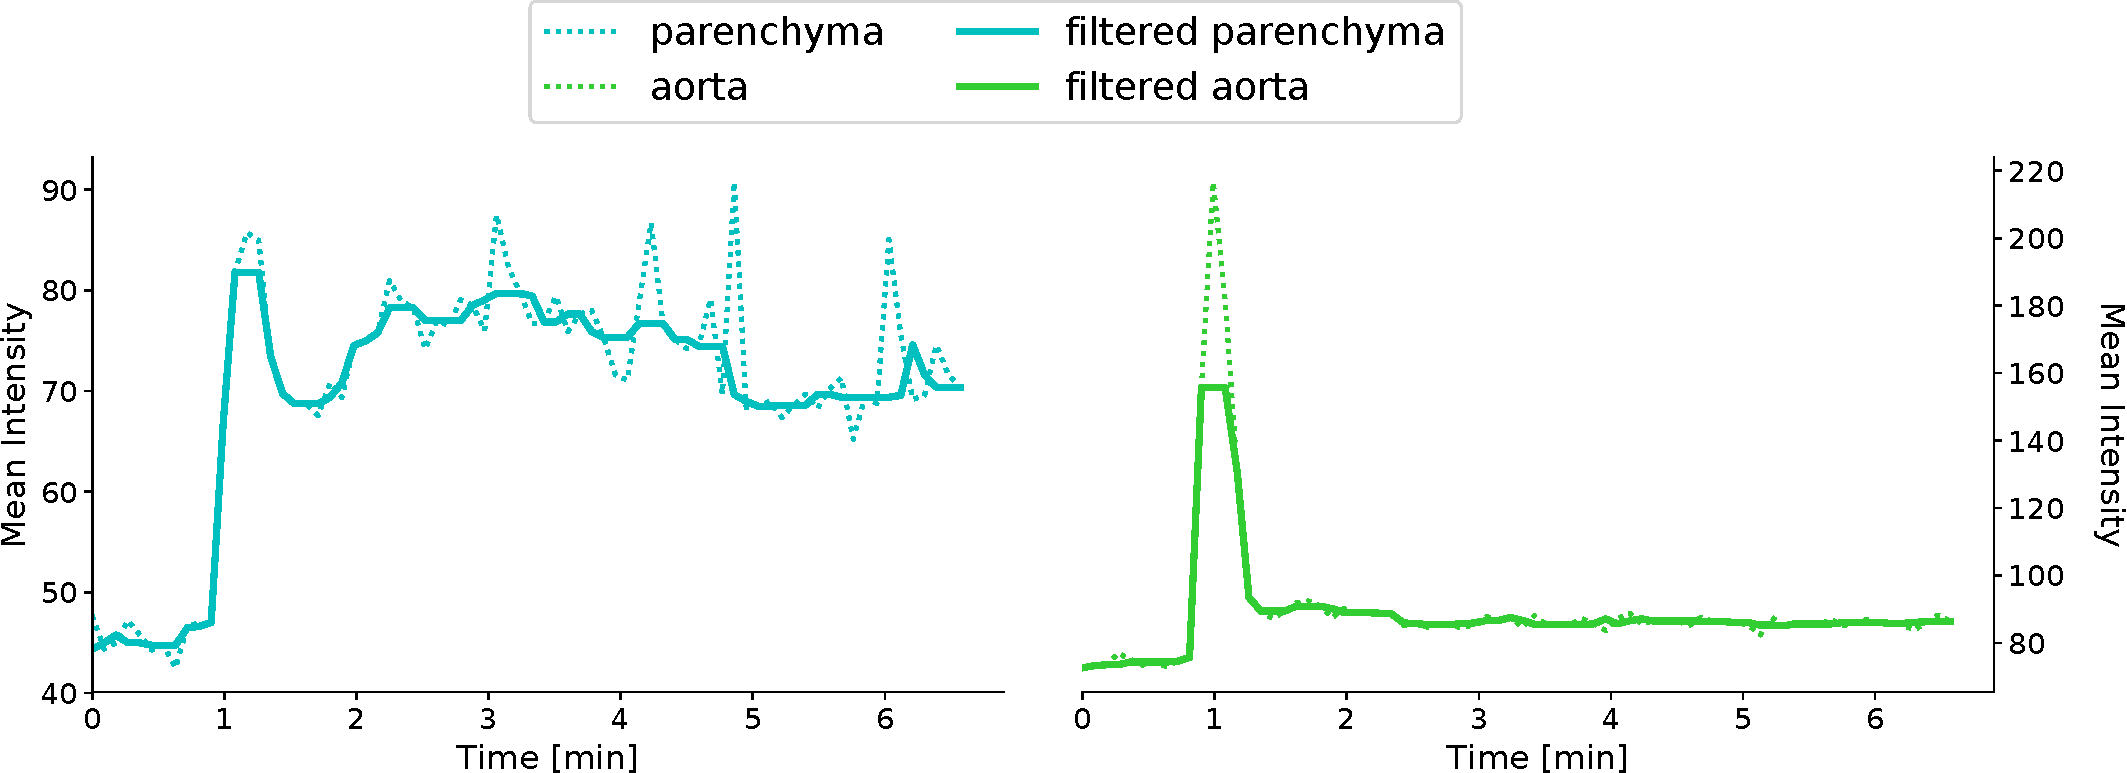
\includegraphics[width = \textwidth]{median2}
\caption[Sample average time-intensity curves for a kidney and aorta with applied median filter]{Sample average time-intensity curves for a kidney and aorta with applied median filter. Note that cut peak of the aorta's signal is a result of the median filter and it is present only during the baseline removal step}
\label{fig:median}
\end{figure}

\begin{figure}[H]
%\captionsetup[subfloat]{captionskip=0.5cm}
	\centering
	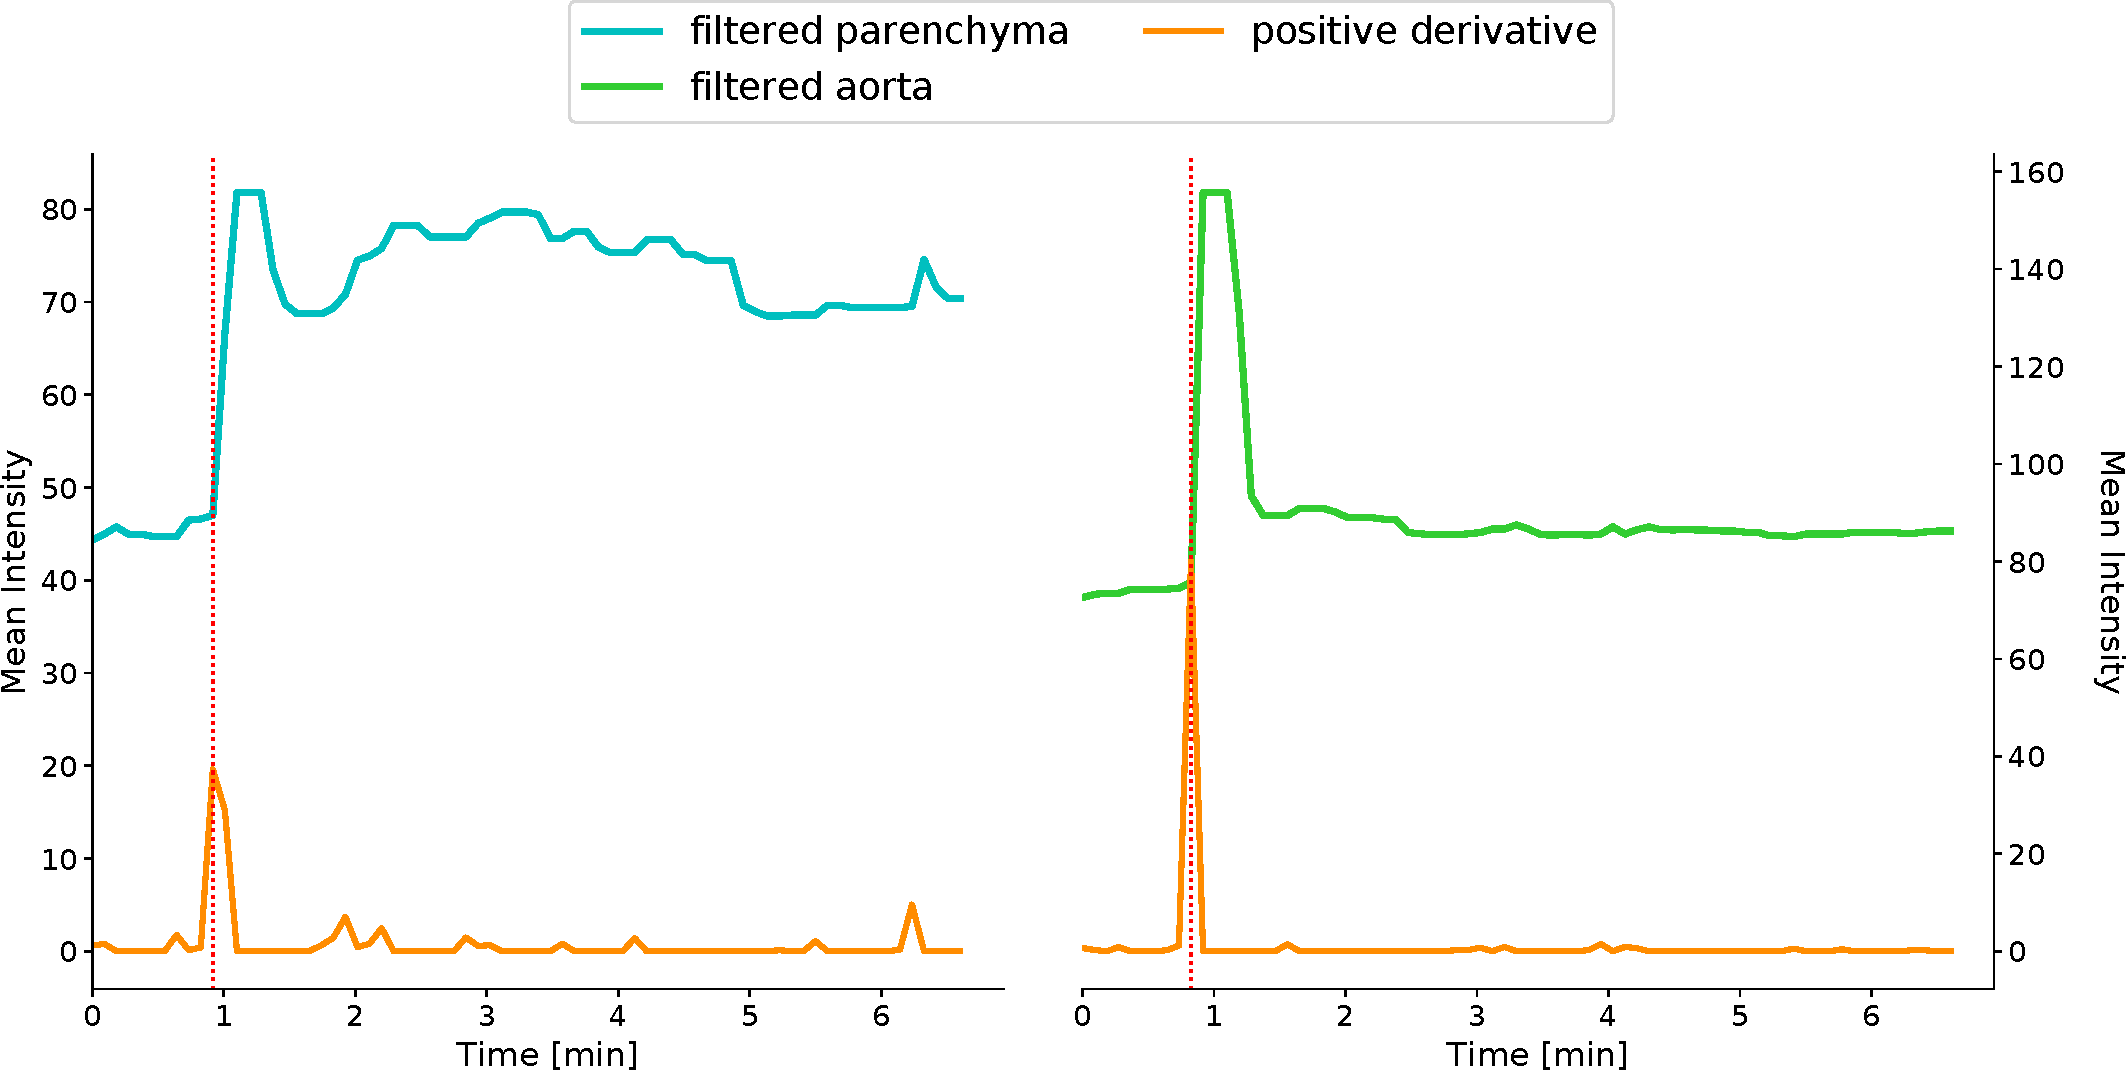
\includegraphics[width = \textwidth]{derivative}
\caption[Positive derivative of the sample kidney and aorta intensity time courses]{Positive derivative of a sample kidney and aorta intensity time courses. The vertical line indicates the time point, in which the derivative reaches its maximal value}
\label{fig:derivative}
\end{figure}

\begin{figure}[H]
%\captionsetup[subfloat]{captionskip=0.5cm}
	\centering
	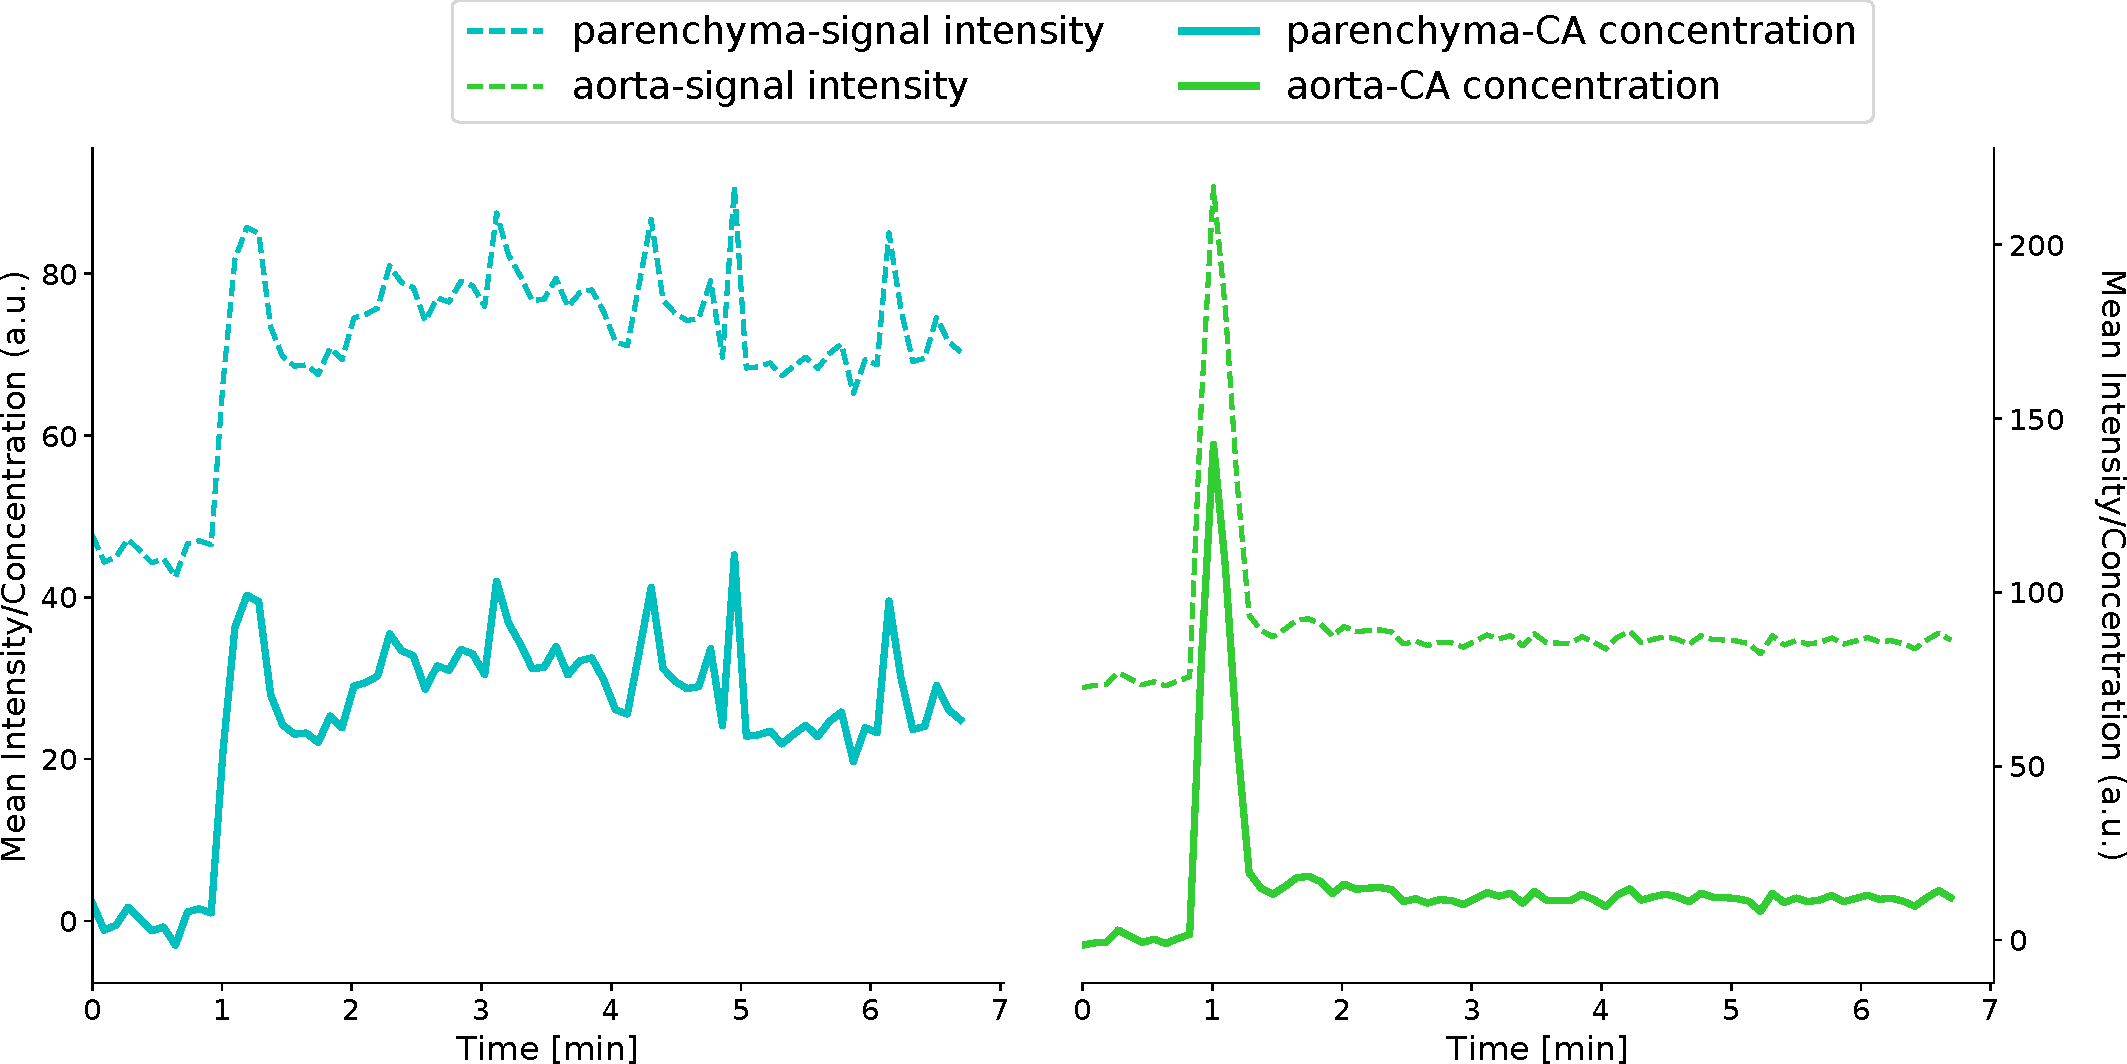
\includegraphics[width = \textwidth]{conversion}
\caption[Time courses of a sample kidney and aorta after intensity-concentration conversion]{Time-intensity curves of a sample kidney and aorta converted into the concentration-time curves}
\label{fig:conversion}
\end{figure}


\subsection{Pharmacokinetic modelling}

Having determined the AIF and the concentration time course for the renal pa\-ren\-chy\-ma, almost all components necessary for the renal quantitative evaluation were obtained. Almost, but not all. One should take into consideration the fact that AIF is the concentration of CA in the blood of the aorta, which consist of both the red blood cells and the blood plasma. Gadolinium-based Contrast Agents, however, distribute in plasma rather than whole blood, so their effective plasma concentrations must be considered. Thus, the \textit{hematocrit} (Hct) correction was performed as follows \cite{tofts2010t1}:
\begin{equation}
	\label{eq:hematocrit}
	C_{p}(t) = \frac{C_{a}(t)} {1-Hct},
\end{equation}
where $C_p$ is CA plasma concentration, $C_a$ is concentration in the aorta defined by the AIF and $Hct$ is the fractional volume of red blood cells in the blood. In this study, its value was taken from the literature as an average population value and was equal to $Hct=0.42$ \cite{tofts2010t1}.

Finally, PK modelling could have been performed. The models of choice were the Tofts and Kermode model, extended Tofts and Kermode model, Patlak-Rutland model and two-compartment exchange model. The aim is to obtain value of the transfer constant $K_{trans}$ [min$^-1$], which corresponds to the GFR per unit tissue volume. The fit was performed by using a non-linear least squares analysis.
 
\paragraph{Tofts and Kermode model.}
According to the \textit{Tofts and Kermode} (TK) model) \cite{tofts1991measurement} the tracer is distributed in two compartments: intravascular and \textit{Extravascular extra-cellular space} (EES).
The tracer diffuses from the blood plasma at rate specified by the transfer constant $K_{trans}$ [min$^{-1}$] and returns at the reverse transfer rate $k_{ep} = K_{trans}/v_e$ [min$^{-1}$]. This model assumes, however, that the amount of intravascular (plasma) tracer is negligible comparing to the tissue signal. 
The tissue concentration, $C_t(t)$, is then given by \cite{khalifa2014models}:
\begin{equation}
C_t(t) = v_eC_e(t),
\end{equation}
\noindent where $v_e$ is EES fractional volume and $C_e(t)$ is EES concentration. The system can be described by mass balance equation  \cite{khalifa2014models, tofts1999estimating}: 
\begin{equation}
	\label{eq:toft}
	\frac{dC_{t}(t)}{dt} = K_{trans}(C_p(t)-C_t(t)/v_e),
\end{equation} 
where  and $C_p(t)$ is blood plasma concentration, The solution obtained according to the procedure presented in Chapter~\ref{chapter:pk} is \cite{sourbron2011scope, khalifa2014models}:
\begin{equation}
	\label{eq:toft2}
	C_{t}(t) =C_p\circledast K_{trans}e^{-k_{ep}t} =K_{trans}\int_{0}^{t}C_p(\tau)e^{-k_{ep}(t-\tau)}d\tau  
\end{equation}
\newpage
\paragraph{Extended Tofts and Keromode model.}
While the Tofts model neglects intravascular contribution assuming weak vascularization of the tissue, the \textit{extended Tofts and Kermode} (ETK) model \cite{tofts1997modeling} does take it into account. According to ETK, the tissue concentration is described by the formula \cite{tofts2010t1, khalifa2014models}:
\begin{equation}
C_t(t) = v_pC_p(t) + v_eC_e(t),
\label{eq:etk}
\end{equation}
where $v_p$ is fractional plasma volume. The differential equation describing the EES compartment is \cite{sourbron2011scope}:
\begin{equation}
	\label{eq:etoft}
	v_e\frac{dC_{e}(t)}{dt} = K_{trans}(C_p(t)-C_e(t))
\end{equation}
Solving the equation and substituting to (\ref{eq:etk}) the tissue concentration boils down to \cite{khalifa2014models, tofts2010t1}:
\begin{align}
	\label{eq:extended_toft}
	C_{t}(t) &=v_pC_p(t) + C_p\circledast K_{trans}e^{-k_{ep}t} =\\
	\nonumber &= v_pC_p(t)+K_{trans}\int_{0}^{t}C_p(\tau)e^{-k_{ep}(t-\tau)}d\tau 
\end{align}


In TK and ETK models the free parameters $K_{trans}$, $v_e$ and $v_p$ are estimated by fitting the model to obtained in DCE-MRI examinations time-concentration curves.  
\paragraph{Patlak-Rutland model.}
Unlike the TK and ETK models, the \textit{Patlak-Rutland} model \cite{patlak1983graphical} assumes that reverse transfer constant from the EES to the plasma, $k_{ep}$, is negligibly small, because of the short time of the measurement (tracer does not have time to return) and low permeability \cite{khalifa2014models}. 
Similarly to the ETK, the tissue concentration is equal to:
\begin{equation}
C_t(t) = v_pC_p(t) + v_eC_e(t)
\label{eq:patlak1}
\end{equation}
\newpage
\noindent However, the tracer change in EES is equal to \cite{thesis,patlak1983graphical}: 
\begin{equation}
	\label{eq:patlak2}
	v_e\frac{dC_{e}(t)}{dt} = K_{trans}C_p(t)
\end{equation}
Solving the Equation (\ref{eq:patlak2}) and substituting into Formula (\ref{eq:patlak2}) \cite{khalifa2014models, patlak1983graphical}: 
\begin{equation}
	\label{eq:patlak}
	C_{t}(t) =v_pC_p(t) + K_{trans}\int_{0}^{t}C_p(\tau)d\tau  
\end{equation}
To obtain the free parameters, the concentration time courses obtained from DCE-MRI examination can be fitted directly to Formula (\ref{eq:patlak}) or the graphical approach called the \textit{Patlak plot} can be applied. In this approach the above equation is linearised as \cite{khalifa2014models, patlak1983graphical}:  
\begin{equation}
	\label{eq:patlak_lin}
	Y = K_{trans}X +v_p,  
\end{equation}
where $Y=C_t(t)/C_p(t)$ and $X=\int_{0}^{t}C_p(\tau)d\tau/C_p(t)$. The free parameters $K_{trans}$ and $v_p$ can be then estimating by constructing a linear plot and calculating its slope and intercept respectively.
In this project, the data was fitted to Formula (\ref{eq:patlak}). 

\paragraph{Two-compartment exchange model.}While all the previously described models allow for estimating transfer constant $K_{trans}$ combining both the plasma blood flow, $F_b$ [min$^{-1}$], and the surface permeability area product, $PS$ [min$^{-1}$], \textit{two-compartment exchange model} (2CXM) enables their separate estimation. 
According to 2CXM, the plasma compartment has an arterial inlet and a venous outlet of the same plasma flow, $Fp$. 
The tracer is exchanged between the two compartments: EES and intravascular plasma, at a symmetric rate quantified by the permeability surface product, $PS$.
Because the CA leaves the system, the model is referred to as an open system. 
Similarly to PR and ETK models the tissue concentration is expressed as \cite{khalifa2014models}:
\begin{equation}
C_t(t) = v_pC_p(t) + v_eC_e(t)
\label{eq:2cxm}
\end{equation}
The system is described by a pair of mass balance differential equations \cite{khalifa2014models}:  
\begin{equation}
v_p\frac{dC_p(t)}{dt} = F_p(C_a(t)-C_p(t))+PS(C_e(t)-C_p(t))
\label{eq:2cxm2}
\end{equation}
\begin{equation}
v_e\frac{dC_e(t)}{dt} = PS(C_p(t)-C_e(t))
\label{eq:2cxm3}
\end{equation}
Note that in 2CXM the CA concentration in the plasma of the feeding artery is denoted as $C_a$ ($C_p$ in previous models) whereas $C_p$ is CA concentration in intravascular plasma. The solution boils down to \cite{khalifa2014models}:
\begin{align}
	\label{eq:2cxm4}
	\nonumber C_{t}(t) &=F_p (Be^{-m_1t}+(1-B)e^{-m_2t})\circledast C_a =\\
	&= F_{p} \int_{0}^{t} \left( Be^{-m_1\tau} + (1-B)e^{-m_2\tau} \right) C_{a}(t-\tau)d\tau
\end{align}
where $m_1$, $m_2$ and $B$ are defined as:
\begin {equation} 
m_1 = \frac{1}{2}\left( a+b+\sqrt{(a+b)^2-4bc}\right)
\end{equation}
\begin {equation} 
\nonumber m_2 = \frac{1}{2}\left(a+b-\sqrt{(a+b)^2-4bc}\right)
\end{equation}
\begin {equation} 
\nonumber B = \frac{m_2-c}{m_2-m_1}, 
\end{equation}
where
\begin{equation}
a = \frac{F_p+PS}{v_p},\qquad b = \frac{PS}{v_e},\qquad c = \frac{F_p}{v_p}
\end{equation}
The $K_{trans}$ can be then obtained by:
\begin{equation}
K_{trans} = \frac{PS\cdot{}F_p}{PS+F_p}
\end{equation}

Sample concentration time course fitted to different models is shown in Figure~\ref{fig:fit}. 

\begin{figure}
\captionsetup[subfloat]{captionskip=0.5cm}
	\centering
	\subfloat[TK model fit; $K_{trans}$ = 0.52 min$^{-1}$ ]{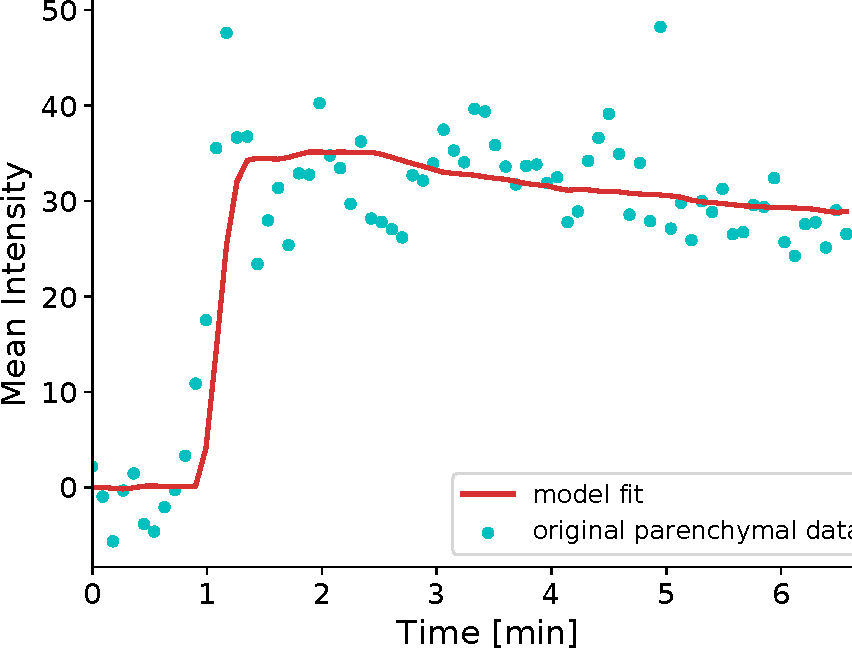
\includegraphics [width=0.48\linewidth]{tk2}}\hspace{0.03\linewidth}
	\subfloat[ETK model fit; $K_{trans}$ = 0.45 min$^{-1}$]{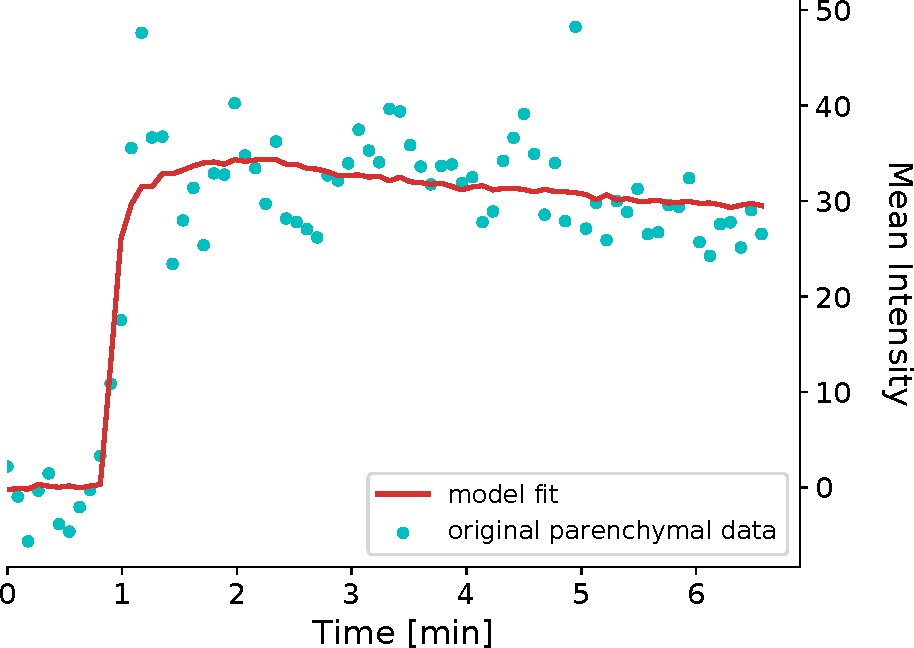
\includegraphics[width=0.48\linewidth]{etk2}}\\ \vspace{1cm}	
	\subfloat[PR model fit; $K_{trans}$ = 0.19 min$^{-1}$]{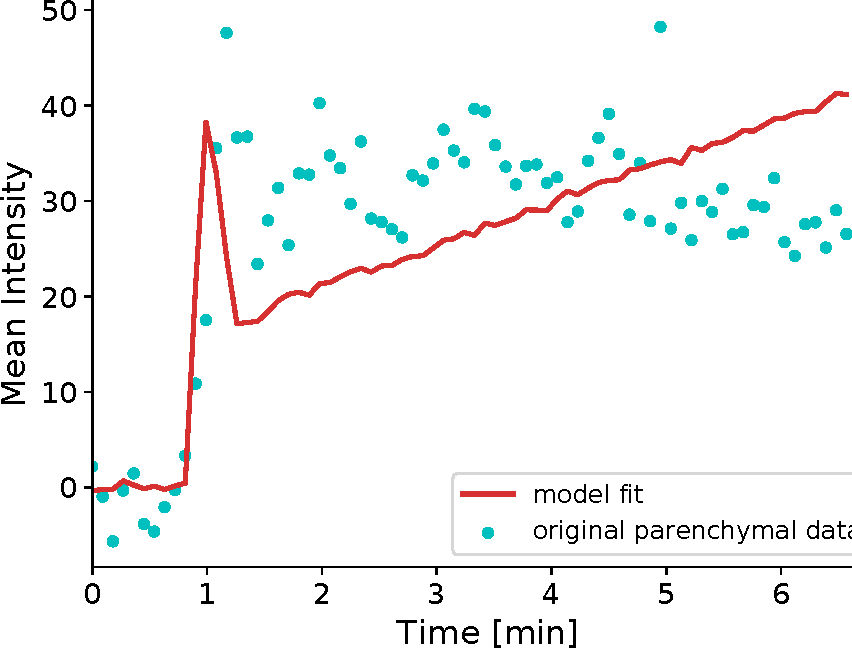
\includegraphics [width=0.48\linewidth]{pr2}}\hspace{0.03\linewidth}
	\subfloat[2CXM model fit; $K_{trans}$ = 0.37 min$^{-1}$]{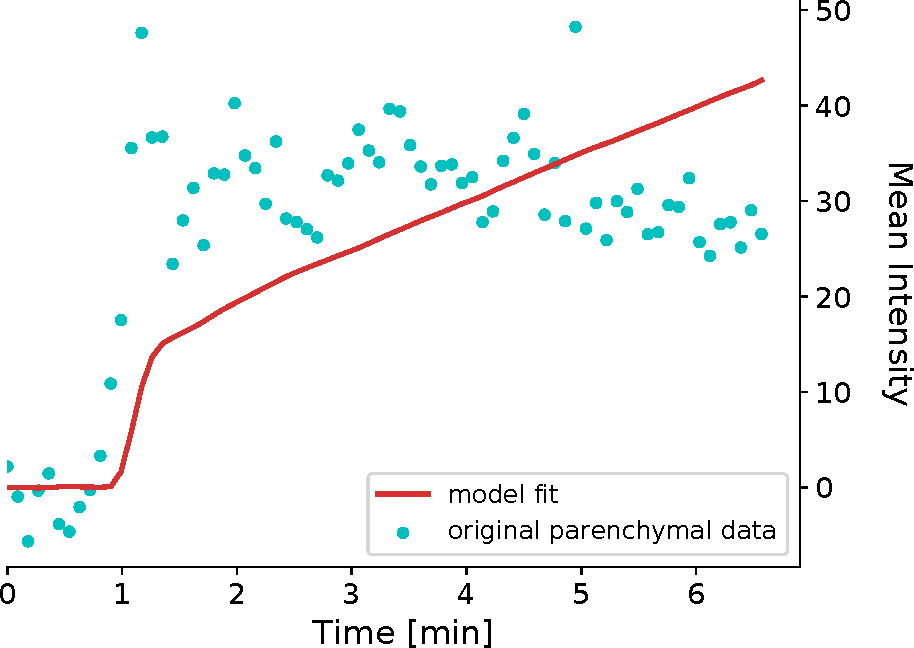
\includegraphics[width=0.48\linewidth]{2cxm2}}\\	
\vspace{1cm}
\caption[An example of models fit]{Sample concentration time course fitted to different PK models: (a) Tofts and Kermode model (b) Extended Tofts and Kermode model (c) Patlak-Rutland model (d) Two-Compartment Exchange Model}
\label{fig:fit}
\end{figure}

\subsection{GFR estimation}
Having estimated the transfer constant $K_{trans}$ the \textit{Single Kidney GFR} (SKGFR) could have been calculated according to the formula:
\begin{equation}
SKGFR = K_{trans}V_{parenchyma},
\end{equation}
where $V_{parenchyma}$ is the parenchymal volume (in mL) of the examined kidney given by:
\begin{equation}
V_{parenchyma} = nV_{voxel},
\end{equation}
where $n$ is the number of voxels included in the kidney label whereas $V_{voxel}$ is the volume of the voxel (2.2\,$\times$\,2.2\,$\times$\,3\,mm$^3$ = 0.14252 mL). Total GFR for each dataset was then calculated by summing up the SKGFR of the left and right kidneys. All obtained GFR values were normalised for standard BSA (1.73\,m$^2$).
